% Created by tikzDevice version 0.10.1 on 2016-08-19 16:51:21
% !TEX encoding = UTF-8 Unicode
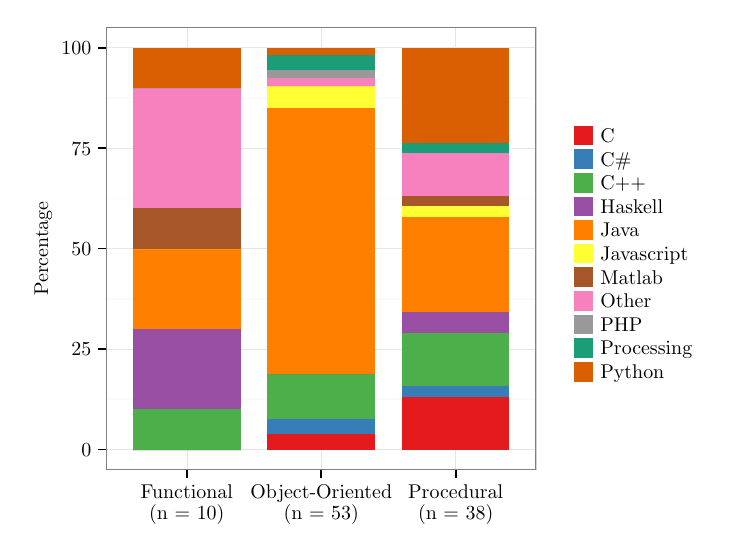
\begin{tikzpicture}[x=1pt,y=1pt]
\definecolor{fillColor}{RGB}{255,255,255}
\path[use as bounding box,fill=fillColor,fill opacity=0.00] (0,0) rectangle (252.94,180.67);
\begin{scope}
\path[clip] (  0.00,  0.00) rectangle (252.94,180.67);
\definecolor{drawColor}{RGB}{255,255,255}
\definecolor{fillColor}{RGB}{255,255,255}

\path[draw=drawColor,line width= 0.6pt,line join=round,line cap=round,fill=fillColor] (  0.00,  0.00) rectangle (252.94,180.68);
\end{scope}
\begin{scope}
\path[clip] ( 28.36, 20.98) rectangle (183.80,180.67);
\definecolor{fillColor}{RGB}{255,255,255}

\path[fill=fillColor] ( 28.36, 20.98) rectangle (183.80,180.67);
\definecolor{drawColor}{gray}{0.98}

\path[draw=drawColor,line width= 0.6pt,line join=round] ( 28.36, 46.39) --
	(183.80, 46.39);

\path[draw=drawColor,line width= 0.6pt,line join=round] ( 28.36, 82.68) --
	(183.80, 82.68);

\path[draw=drawColor,line width= 0.6pt,line join=round] ( 28.36,118.97) --
	(183.80,118.97);

\path[draw=drawColor,line width= 0.6pt,line join=round] ( 28.36,155.27) --
	(183.80,155.27);
\definecolor{drawColor}{gray}{0.90}

\path[draw=drawColor,line width= 0.2pt,line join=round] ( 28.36, 28.24) --
	(183.80, 28.24);

\path[draw=drawColor,line width= 0.2pt,line join=round] ( 28.36, 64.53) --
	(183.80, 64.53);

\path[draw=drawColor,line width= 0.2pt,line join=round] ( 28.36,100.83) --
	(183.80,100.83);

\path[draw=drawColor,line width= 0.2pt,line join=round] ( 28.36,137.12) --
	(183.80,137.12);

\path[draw=drawColor,line width= 0.2pt,line join=round] ( 28.36,173.42) --
	(183.80,173.42);

\path[draw=drawColor,line width= 0.2pt,line join=round] ( 57.50, 20.98) --
	( 57.50,180.67);

\path[draw=drawColor,line width= 0.2pt,line join=round] (106.08, 20.98) --
	(106.08,180.67);

\path[draw=drawColor,line width= 0.2pt,line join=round] (154.66, 20.98) --
	(154.66,180.67);
\definecolor{fillColor}{RGB}{228,26,28}

\path[fill=fillColor] ( 38.07, 28.24) rectangle ( 76.93, 28.24);
\definecolor{fillColor}{RGB}{55,126,184}

\path[fill=fillColor] ( 38.07, 28.24) rectangle ( 76.93, 28.24);
\definecolor{fillColor}{RGB}{77,175,74}

\path[fill=fillColor] ( 38.07, 28.24) rectangle ( 76.93, 42.76);
\definecolor{fillColor}{RGB}{152,78,163}

\path[fill=fillColor] ( 38.07, 42.76) rectangle ( 76.93, 71.79);
\definecolor{fillColor}{RGB}{255,127,0}

\path[fill=fillColor] ( 38.07, 71.79) rectangle ( 76.93,100.83);
\definecolor{fillColor}{RGB}{255,255,51}

\path[fill=fillColor] ( 38.07,100.83) rectangle ( 76.93,100.83);
\definecolor{fillColor}{RGB}{166,86,40}

\path[fill=fillColor] ( 38.07,100.83) rectangle ( 76.93,115.35);
\definecolor{fillColor}{RGB}{247,129,191}

\path[fill=fillColor] ( 38.07,115.35) rectangle ( 76.93,158.90);
\definecolor{fillColor}{gray}{0.60}

\path[fill=fillColor] ( 38.07,158.90) rectangle ( 76.93,158.90);
\definecolor{fillColor}{RGB}{27,158,119}

\path[fill=fillColor] ( 38.07,158.90) rectangle ( 76.93,158.90);
\definecolor{fillColor}{RGB}{217,95,2}

\path[fill=fillColor] ( 38.07,158.90) rectangle ( 76.93,173.42);
\definecolor{fillColor}{RGB}{228,26,28}

\path[fill=fillColor] ( 86.65, 28.24) rectangle (125.51, 33.72);
\definecolor{fillColor}{RGB}{55,126,184}

\path[fill=fillColor] ( 86.65, 33.72) rectangle (125.51, 39.20);
\definecolor{fillColor}{RGB}{77,175,74}

\path[fill=fillColor] ( 86.65, 39.20) rectangle (125.51, 55.63);
\definecolor{fillColor}{RGB}{152,78,163}

\path[fill=fillColor] ( 86.65, 55.63) rectangle (125.51, 55.63);
\definecolor{fillColor}{RGB}{255,127,0}

\path[fill=fillColor] ( 86.65, 55.63) rectangle (125.51,151.50);
\definecolor{fillColor}{RGB}{255,255,51}

\path[fill=fillColor] ( 86.65,151.50) rectangle (125.51,159.72);
\definecolor{fillColor}{RGB}{166,86,40}

\path[fill=fillColor] ( 86.65,159.72) rectangle (125.51,159.72);
\definecolor{fillColor}{RGB}{247,129,191}

\path[fill=fillColor] ( 86.65,159.72) rectangle (125.51,162.46);
\definecolor{fillColor}{gray}{0.60}

\path[fill=fillColor] ( 86.65,162.46) rectangle (125.51,165.20);
\definecolor{fillColor}{RGB}{27,158,119}

\path[fill=fillColor] ( 86.65,165.20) rectangle (125.51,170.68);
\definecolor{fillColor}{RGB}{217,95,2}

\path[fill=fillColor] ( 86.65,170.68) rectangle (125.51,173.42);
\definecolor{fillColor}{RGB}{228,26,28}

\path[fill=fillColor] (135.23, 28.24) rectangle (174.09, 47.34);
\definecolor{fillColor}{RGB}{55,126,184}

\path[fill=fillColor] (135.23, 47.34) rectangle (174.09, 51.16);
\definecolor{fillColor}{RGB}{77,175,74}

\path[fill=fillColor] (135.23, 51.16) rectangle (174.09, 70.26);
\definecolor{fillColor}{RGB}{152,78,163}

\path[fill=fillColor] (135.23, 70.26) rectangle (174.09, 77.90);
\definecolor{fillColor}{RGB}{255,127,0}

\path[fill=fillColor] (135.23, 77.90) rectangle (174.09,112.29);
\definecolor{fillColor}{RGB}{255,255,51}

\path[fill=fillColor] (135.23,112.29) rectangle (174.09,116.11);
\definecolor{fillColor}{RGB}{166,86,40}

\path[fill=fillColor] (135.23,116.11) rectangle (174.09,119.93);
\definecolor{fillColor}{RGB}{247,129,191}

\path[fill=fillColor] (135.23,119.93) rectangle (174.09,135.21);
\definecolor{fillColor}{gray}{0.60}

\path[fill=fillColor] (135.23,135.21) rectangle (174.09,135.21);
\definecolor{fillColor}{RGB}{27,158,119}

\path[fill=fillColor] (135.23,135.21) rectangle (174.09,139.03);
\definecolor{fillColor}{RGB}{217,95,2}

\path[fill=fillColor] (135.23,139.03) rectangle (174.09,173.42);
\definecolor{drawColor}{gray}{0.50}

\path[draw=drawColor,line width= 0.6pt,line join=round,line cap=round] ( 28.36, 20.98) rectangle (183.80,180.67);
\end{scope}
\begin{scope}
\path[clip] (  0.00,  0.00) rectangle (252.94,180.67);
\definecolor{drawColor}{RGB}{0,0,0}

\node[text=drawColor,anchor=base east,inner sep=0pt, outer sep=0pt, scale=  0.72] at ( 22.96, 25.76) {0};

\node[text=drawColor,anchor=base east,inner sep=0pt, outer sep=0pt, scale=  0.72] at ( 22.96, 62.05) {25};

\node[text=drawColor,anchor=base east,inner sep=0pt, outer sep=0pt, scale=  0.72] at ( 22.96, 98.35) {50};

\node[text=drawColor,anchor=base east,inner sep=0pt, outer sep=0pt, scale=  0.72] at ( 22.96,134.64) {75};

\node[text=drawColor,anchor=base east,inner sep=0pt, outer sep=0pt, scale=  0.72] at ( 22.96,170.94) {100};
\end{scope}
\begin{scope}
\path[clip] (  0.00,  0.00) rectangle (252.94,180.67);
\definecolor{drawColor}{RGB}{0,0,0}

\path[draw=drawColor,line width= 0.6pt,line join=round] ( 25.36, 28.24) --
	( 28.36, 28.24);

\path[draw=drawColor,line width= 0.6pt,line join=round] ( 25.36, 64.53) --
	( 28.36, 64.53);

\path[draw=drawColor,line width= 0.6pt,line join=round] ( 25.36,100.83) --
	( 28.36,100.83);

\path[draw=drawColor,line width= 0.6pt,line join=round] ( 25.36,137.12) --
	( 28.36,137.12);

\path[draw=drawColor,line width= 0.6pt,line join=round] ( 25.36,173.42) --
	( 28.36,173.42);
\end{scope}
\begin{scope}
\path[clip] (  0.00,  0.00) rectangle (252.94,180.67);
\definecolor{drawColor}{RGB}{0,0,0}

\path[draw=drawColor,line width= 0.6pt,line join=round] ( 57.50, 17.98) --
	( 57.50, 20.98);

\path[draw=drawColor,line width= 0.6pt,line join=round] (106.08, 17.98) --
	(106.08, 20.98);

\path[draw=drawColor,line width= 0.6pt,line join=round] (154.66, 17.98) --
	(154.66, 20.98);
\end{scope}
\begin{scope}
\path[clip] (  0.00,  0.00) rectangle (252.94,180.67);
\definecolor{drawColor}{RGB}{0,0,0}

\node[text=drawColor,anchor=base,inner sep=0pt, outer sep=0pt, scale=  0.72] at ( 57.50, 10.62) {Functional};

\node[text=drawColor,anchor=base,inner sep=0pt, outer sep=0pt, scale=  0.72] at ( 57.50,  2.85) {(n = 10)};

\node[text=drawColor,anchor=base,inner sep=0pt, outer sep=0pt, scale=  0.72] at (106.08, 10.62) {Object-Oriented};

\node[text=drawColor,anchor=base,inner sep=0pt, outer sep=0pt, scale=  0.72] at (106.08,  2.85) {(n = 53)};

\node[text=drawColor,anchor=base,inner sep=0pt, outer sep=0pt, scale=  0.72] at (154.66, 10.62) {Procedural};

\node[text=drawColor,anchor=base,inner sep=0pt, outer sep=0pt, scale=  0.72] at (154.66,  2.85) {(n = 38)};
\end{scope}
\begin{scope}
\path[clip] (  0.00,  0.00) rectangle (252.94,180.67);
\definecolor{drawColor}{RGB}{0,0,0}

\node[text=drawColor,rotate= 90.00,anchor=base,inner sep=0pt, outer sep=0pt, scale=  0.72] at (  7.36,100.83) {Percentage};
\end{scope}
\begin{scope}
\path[clip] (  0.00,  0.00) rectangle (252.94,180.67);
\definecolor{fillColor}{RGB}{255,255,255}

\path[fill=fillColor] (192.34, 47.81) rectangle (244.41,153.85);
\end{scope}
\begin{scope}
\path[clip] (  0.00,  0.00) rectangle (252.94,180.67);
\definecolor{fillColor}{RGB}{228,26,28}

\path[fill=fillColor] (197.32,138.14) rectangle (204.43,145.26);
\end{scope}
\begin{scope}
\path[clip] (  0.00,  0.00) rectangle (252.94,180.67);
\definecolor{fillColor}{RGB}{55,126,184}

\path[fill=fillColor] (197.32,129.61) rectangle (204.43,136.72);
\end{scope}
\begin{scope}
\path[clip] (  0.00,  0.00) rectangle (252.94,180.67);
\definecolor{fillColor}{RGB}{77,175,74}

\path[fill=fillColor] (197.32,121.07) rectangle (204.43,128.18);
\end{scope}
\begin{scope}
\path[clip] (  0.00,  0.00) rectangle (252.94,180.67);
\definecolor{fillColor}{RGB}{152,78,163}

\path[fill=fillColor] (197.32,112.54) rectangle (204.43,119.65);
\end{scope}
\begin{scope}
\path[clip] (  0.00,  0.00) rectangle (252.94,180.67);
\definecolor{fillColor}{RGB}{255,127,0}

\path[fill=fillColor] (197.32,104.00) rectangle (204.43,111.11);
\end{scope}
\begin{scope}
\path[clip] (  0.00,  0.00) rectangle (252.94,180.67);
\definecolor{fillColor}{RGB}{255,255,51}

\path[fill=fillColor] (197.32, 95.46) rectangle (204.43,102.58);
\end{scope}
\begin{scope}
\path[clip] (  0.00,  0.00) rectangle (252.94,180.67);
\definecolor{fillColor}{RGB}{166,86,40}

\path[fill=fillColor] (197.32, 86.93) rectangle (204.43, 94.04);
\end{scope}
\begin{scope}
\path[clip] (  0.00,  0.00) rectangle (252.94,180.67);
\definecolor{fillColor}{RGB}{247,129,191}

\path[fill=fillColor] (197.32, 78.39) rectangle (204.43, 85.51);
\end{scope}
\begin{scope}
\path[clip] (  0.00,  0.00) rectangle (252.94,180.67);
\definecolor{fillColor}{gray}{0.60}

\path[fill=fillColor] (197.32, 69.86) rectangle (204.43, 76.97);
\end{scope}
\begin{scope}
\path[clip] (  0.00,  0.00) rectangle (252.94,180.67);
\definecolor{fillColor}{RGB}{27,158,119}

\path[fill=fillColor] (197.32, 61.32) rectangle (204.43, 68.43);
\end{scope}
\begin{scope}
\path[clip] (  0.00,  0.00) rectangle (252.94,180.67);
\definecolor{fillColor}{RGB}{217,95,2}

\path[fill=fillColor] (197.32, 52.79) rectangle (204.43, 59.90);
\end{scope}
\begin{scope}
\path[clip] (  0.00,  0.00) rectangle (252.94,180.67);
\definecolor{drawColor}{RGB}{0,0,0}

\node[text=drawColor,anchor=base west,inner sep=0pt, outer sep=0pt, scale=  0.72] at (206.95,139.22) {C};
\end{scope}
\begin{scope}
\path[clip] (  0.00,  0.00) rectangle (252.94,180.67);
\definecolor{drawColor}{RGB}{0,0,0}

\node[text=drawColor,anchor=base west,inner sep=0pt, outer sep=0pt, scale=  0.72] at (206.95,130.68) {C\#};
\end{scope}
\begin{scope}
\path[clip] (  0.00,  0.00) rectangle (252.94,180.67);
\definecolor{drawColor}{RGB}{0,0,0}

\node[text=drawColor,anchor=base west,inner sep=0pt, outer sep=0pt, scale=  0.72] at (206.95,122.15) {C++};
\end{scope}
\begin{scope}
\path[clip] (  0.00,  0.00) rectangle (252.94,180.67);
\definecolor{drawColor}{RGB}{0,0,0}

\node[text=drawColor,anchor=base west,inner sep=0pt, outer sep=0pt, scale=  0.72] at (206.95,113.61) {Haskell};
\end{scope}
\begin{scope}
\path[clip] (  0.00,  0.00) rectangle (252.94,180.67);
\definecolor{drawColor}{RGB}{0,0,0}

\node[text=drawColor,anchor=base west,inner sep=0pt, outer sep=0pt, scale=  0.72] at (206.95,105.08) {Java};
\end{scope}
\begin{scope}
\path[clip] (  0.00,  0.00) rectangle (252.94,180.67);
\definecolor{drawColor}{RGB}{0,0,0}

\node[text=drawColor,anchor=base west,inner sep=0pt, outer sep=0pt, scale=  0.72] at (206.95, 96.54) {Javascript};
\end{scope}
\begin{scope}
\path[clip] (  0.00,  0.00) rectangle (252.94,180.67);
\definecolor{drawColor}{RGB}{0,0,0}

\node[text=drawColor,anchor=base west,inner sep=0pt, outer sep=0pt, scale=  0.72] at (206.95, 88.01) {Matlab};
\end{scope}
\begin{scope}
\path[clip] (  0.00,  0.00) rectangle (252.94,180.67);
\definecolor{drawColor}{RGB}{0,0,0}

\node[text=drawColor,anchor=base west,inner sep=0pt, outer sep=0pt, scale=  0.72] at (206.95, 79.47) {Other};
\end{scope}
\begin{scope}
\path[clip] (  0.00,  0.00) rectangle (252.94,180.67);
\definecolor{drawColor}{RGB}{0,0,0}

\node[text=drawColor,anchor=base west,inner sep=0pt, outer sep=0pt, scale=  0.72] at (206.95, 70.93) {PHP};
\end{scope}
\begin{scope}
\path[clip] (  0.00,  0.00) rectangle (252.94,180.67);
\definecolor{drawColor}{RGB}{0,0,0}

\node[text=drawColor,anchor=base west,inner sep=0pt, outer sep=0pt, scale=  0.72] at (206.95, 62.40) {Processing};
\end{scope}
\begin{scope}
\path[clip] (  0.00,  0.00) rectangle (252.94,180.67);
\definecolor{drawColor}{RGB}{0,0,0}

\node[text=drawColor,anchor=base west,inner sep=0pt, outer sep=0pt, scale=  0.72] at (206.95, 53.86) {Python};
\end{scope}
\end{tikzpicture}
